\vspace{1cm}

\noindent \textbf{\Large Lista de Exercícios 12 — Tópicos Avançados (Exceções, NumPy, Pandas e Matplotlib)}

\vspace{0.3cm}
\noindent \textbf{Orientações e Instruções Gerais:}
\begin{itemize}[leftmargin=*]
    \item Esta lista consolida os tópicos avançados ministrados entre as \textbf{Aulas 12 e 15} da disciplina, totalizando \textbf{100,0 pontos} (10 questões de 10,0 pontos cada).
    \item \textbf{Formato e Entrega:} As resoluções devem ser desenvolvidas em Python e entregues em formato Jupyter Notebook (\texttt{.ipynb}) ou Google Colab na plataforma Google Classroom.
    \item Para questões de implementação, respeite rigorosamente os protótipos fornecidos, nomes de funções, parâmetros e \textbf{Type Hints}.
    \item Priorize o uso dos paradigmas oficiais das bibliotecas: tratamento especializado de exceções, operações vetorizadas no NumPy (evitando laços desnecessários), manipulação tabular no Pandas com métodos nativos e construção gráfica orientada a objetos no Matplotlib (\texttt{fig, ax = plt.subplots()}).
\end{itemize}

\vspace{0.5cm}

\begin{enumerate}[label=\textbf{Q\arabic*.}]

% Q1 - Aula 12: try, except, else, finally
\item \textbf{[Discursiva - 10,0 pontos]} Em um sistema de Guerra Acústica, boias hidrofônicas transmitem pacotes de telemetria contendo dados numéricos brutos em formatos textuais heterogêneos. Algumas transmissões apresentam falhas de rede que geram chaves ausentes, caracteres inválidos ou divisões proibidas por zero.

Escreva a função \code{processar\_pacote\_sonar(pacote: Dict[str, Any], log\_execucao: List[str]) -> Dict[str, float]} que processe um pacote de telemetria aplicando tratamento robusto de exceções:
\begin{itemize}[leftmargin=*]
    \item \textbf{1.} No bloco \code{try}, converta \code{pacote["frequencia\_hz"]} e \code{pacote["amplitude\_db"]} para \code{float}. Caso a frequência seja menor ou igual a zero ($\le 0$), dispare intencionalmente um \code{ValueError("Frequência deve ser estritamente positiva.")}.
    \item \textbf{2.} Calcule a razão de sinal: $\text{razao} = \frac{\text{amplitude\_db}}{\text{frequencia\_hz}}$. Retorne um dicionário contendo \code{"frequencia\_hz"}, \code{"amplitude\_db"} e \code{"razao\_sinal"} (arredondada para 4 casas decimais).
    \item \textbf{3.} Capture de forma especializada:
    \begin{itemize}
        \item \code{KeyError}: anexe a string \code{"ERRO\_CHAVE\_AUSENTE: <msg>"} na lista \code{log\_execucao}.
        \item \code{(ValueError, TypeError)}: anexe a string \code{"ERRO\_VALOR\_INVALIDO: <msg>"} na lista \code{log\_execucao}.
        \item \code{ZeroDivisionError}: anexe a string \code{"ERRO\_DIVISAO\_ZERO: <msg>"} na lista \code{log\_execucao}.
    \end{itemize}
    Em qualquer caso de exceção capturada, a função deve retornar o dicionário zerado: \code{\{"frequencia\_hz": 0.0, "amplitude\_db": 0.0, "razao\_sinal": 0.0\}}.
    \item \textbf{4.} No bloco \code{else}, anexe a string \code{"SUCESSO\_PROCESSAMENTO"} na lista \code{log\_execucao}.
    \item \textbf{5.} No bloco \code{finally}, anexe obrigatoriamente a string \code{"PACOTE\_FINALIZADO"} na lista \code{log\_execucao}.
\end{itemize}

\begin{itemize}[leftmargin=*]
    \item \textbf{Protótipo:}\newline
    \code{from typing import Dict, Any, List}\\\code{def processar\_pacote\_sonar(}\\\code{    pacote: Dict[str, Any],}\\\code{    log\_execucao: List[str]}\\\code{) -> Dict[str, float]:}
    \item \textbf{Exemplo de Entrada Válida:}\newline
    \code{pacote = \{"frequencia\_hz": "250.0", "amplitude\_db": 50.0\}}\newline
    \textbf{Saída:}\newline
    \code{\{"frequencia\_hz": 250.0, "amplitude\_db": 50.0, "razao\_sinal": 0.2\}}\newline
    \code{log\_execucao = ["SUCESSO\_PROCESSAMENTO", "PACOTE\_FINALIZADO"]}
\end{itemize}

\ifmostrarGabarito
\begin{minted}{python}
from typing import Dict, Any, List

def processar_pacote_sonar(pacote: Dict[str, Any], log_execucao: List[str]) -> Dict[str, float]:
    """
    Processa e normaliza um pacote de telemetria acústica com tratamento robusto de erros.
    """
    resultado = {"frequencia_hz": 0.0, "amplitude_db": 0.0, "razao_sinal": 0.0}
    try:
        freq = float(pacote["frequencia_hz"])
        amp = float(pacote["amplitude_db"])
        
        if freq <= 0:
            raise ValueError("Frequência deve ser estritamente positiva.")
            
        razao = amp / freq
        resultado = {
            "frequencia_hz": round(freq, 2),
            "amplitude_db": round(amp, 2),
            "razao_sinal": round(razao, 4)
        }
    except KeyError as e:
        log_execucao.append(f"ERRO_CHAVE_AUSENTE: {e}")
    except (ValueError, TypeError) as e:
        log_execucao.append(f"ERRO_VALOR_INVALIDO: {e}")
    except ZeroDivisionError as e:
        log_execucao.append(f"ERRO_DIVISAO_ZERO: {e}")
    else:
        log_execucao.append("SUCESSO_PROCESSAMENTO")
    finally:
        log_execucao.append("PACOTE_FINALIZADO")
        
    return resultado
\end{minted}

\textbf{Explicação:}
A função implementa a estrutura completa de tratamento de exceções em Python:
\begin{itemize}[leftmargin=*]
    \item \texttt{try}: Tenta converter as entradas numéricas, calcula a métrica derivada e valida se a frequência é positiva.
    \item \texttt{except}: Captura de forma especializada erros de chave ausente (\texttt{KeyError}), problemas de tipo/valor (\texttt{ValueError}, \texttt{TypeError}) e divisão por zero (\texttt{ZeroDivisionError}), registrando a falha no log.
    \item \texttt{else}: Executado exclusivamente quando nenhuma exceção é levantada, confirmando o sucesso da operação.
    \item \texttt{finally}: Executado incondicionalmente em todos os cenários, assegurando que o encerramento do pacote fique auditado no log.
\end{itemize}
\fi


\vspace{0.5cm}

% Q2 - Aula 12: Exceções Personalizadas e raise
\item \textbf{[Discursiva - 10,0 pontos]} O subsistema de propulsão de um submarino de ataque exige validações de segurança em tempo real antes que qualquer manobra tática evasiva seja iniciada. Crie uma estrutura orientada a objetos de exceções personalizadas e as respectivas funções de validação:

\begin{itemize}[leftmargin=*]
    \item \textbf{1. Hierarquia de Exceções:}\newline
    Crie a classe base \code{FalhaPropulsaoError(Exception)} e duas subclasses derivadas: \code{CombustivelInsuficienteError(FalhaPropulsaoError)} e \code{SobreaquecimentoTurbinaError(FalhaPropulsaoError)}.
    \item \textbf{2. Função de Validação com \code{raise}:}\newline
    Implemente a função \code{autorizar\_manobra\_tatica(combustivel\_atual: float, consumo\_previsto: float, temp\_turbina: float, temp\_maxima: float) -> bool}:
    \begin{itemize}
        \item Se $\text{consumo\_previsto} > \text{combustivel\_atual}$, dispare \code{CombustivelInsuficienteError} com mensagem detalhada.
        \item Se $\text{temp\_turbina} > \text{temp\_maxima}$, dispare \code{SobreaquecimentoTurbinaError} com mensagem detalhada.
        \item Se nenhuma condição for violada, retorne \code{True}.
    \end{itemize}
    \item \textbf{3. Função de Supervisão Operacional:}\newline
    Implemente a função \code{executar\_verificacao\_manobra(...)} que chame a função anterior dentro de um bloco \code{try/except}. Se a manobra for válida, retorne a tupla \code{(True, "MANOBRA\_AUTORIZADA")}. Caso contrário, capture as exceções especificamente e retorne \code{(False, "<MOTIVO\_DO\_ERRO>")}.
\end{itemize}

\begin{itemize}[leftmargin=*]
    \item \textbf{Protótipos:}\newline
    \code{class FalhaPropulsaoError(Exception): pass}\newline
    \code{class CombustivelInsuficienteError(FalhaPropulsaoError): pass}\newline
    \code{class SobreaquecimentoTurbinaError(FalhaPropulsaoError): pass}\newline
    \code{from typing import Tuple}\\\code{def autorizar\_manobra\_tatica(}\\\code{    combustivel\_atual: float, consumo\_previsto: float,}\\\code{    temp\_turbina: float, temp\_maxima: float}\\\code{) -> bool:}\newline
    \code{def executar\_verificacao\_manobra(}\\\code{    combustivel\_atual: float, consumo\_previsto: float,}\\\code{    temp\_turbina: float, temp\_maxima: float}\\\code{) -> Tuple[bool, str]:}
    \item \textbf{Exemplo de Falha de Temperatura:}\newline
    \code{executar\_verificacao\_manobra(1000.0, 300.0, 920.0, 850.0)}\newline
    $\rightarrow$ \code{(False, "FALHA\_TEMPERATURA: Temperatura critica: 920.0C excede teto seguro de 850.0C.")}
\end{itemize}

\ifmostrarGabarito
\begin{minted}{python}
from typing import Tuple

class FalhaPropulsaoError(Exception):
    """Classe base para falhas do sistema de propulsão."""
    pass

class CombustivelInsuficienteError(FalhaPropulsaoError):
    """Disparada quando o combustível não atende ao consumo previsto."""
    pass

class SobreaquecimentoTurbinaError(FalhaPropulsaoError):
    """Disparada quando a temperatura da turbina supera o teto de segurança."""
    pass


def autorizar_manobra_tatica(
    combustivel_atual: float,
    consumo_previsto: float,
    temp_turbina: float,
    temp_maxima: float
) -> bool:
    """
    Avalia a segurança de manobra e dispara exceções personalizadas em caso de risco.
    """
    if consumo_previsto > combustivel_atual:
        raise CombustivelInsuficienteError(
            f"Combustivel insuficiente: requerido {consumo_previsto:.1f}L, disponivel {combustivel_atual:.1f}L."
        )
    if temp_turbina > temp_maxima:
        raise SobreaquecimentoTurbinaError(
            f"Temperatura critica: {temp_turbina:.1f}C excede teto seguro de {temp_maxima:.1f}C."
        )
    return True


def executar_verificacao_manobra(
    combustivel_atual: float,
    consumo_previsto: float,
    temp_turbina: float,
    temp_maxima: float
) -> Tuple[bool, str]:
    """
    Invoca a verificação e captura as exceções personalizadas com mensagens adequadas.
    """
    try:
        autorizar_manobra_tatica(combustivel_atual, consumo_previsto, temp_turbina, temp_maxima)
        return (True, "MANOBRA_AUTORIZADA")
    except CombustivelInsuficienteError as err:
        return (False, f"FALHA_COMBUSTIVEL: {err}")
    except SobreaquecimentoTurbinaError as err:
        return (False, f"FALHA_TEMPERATURA: {err}")
    except FalhaPropulsaoError as err:
        return (False, f"FALHA_PROPULSAO_GENERICA: {err}")
\end{minted}

\textbf{Explicação:}
A solução modela a hierarquia orientada a objetos de exceções customizadas herdando de \texttt{Exception}. A função \texttt{autorizar\_manobra\_tatica} utiliza \texttt{raise} para interromper o fluxo quando parâmetros críticos são violados. A função de supervisão \texttt{executar\_verificacao\_manobra} captura especificamente cada exceção filha antes da classe base, permitindo tratamento diferenciado e seguro.
\fi


\vspace{0.5cm}

% Q3 - Aula 13: NumPy Vetorização, Máscaras e np.where
\item \textbf{[Discursiva - 10,0 pontos]} No pré-processamento digital de sinais capturados por uma cortina de hidrofones, é fundamental atenuar o ruído ambiente de fundo e destacar contatos de alta energia.

Utilizando exclusivamente recursos vetorizados do \textbf{NumPy} (é terminantemente proibido o uso de laços \code{for} ou \code{while}), escreva a função \code{filtrar\_sinal\_hidrofone(leituras\_brutas: np.ndarray, limiar\_ruido: float, fator\_ganho: float) -> Tuple[np.ndarray, int]}:
\begin{itemize}[leftmargin=*]
    \item Construa uma máscara booleana vetorizada que identifique todas as amostras cujo valor absoluto seja maior ou igual ao limiar de ruído ($|\text{leitura}| \ge \text{limiar\_ruido}$).
    \item Com a função \code{np.where()}, gere um novo array no qual as amostras que superam o limiar sejam multiplicadas pelo \code{fator\_ganho}, e as amostras inferiores ao limiar sejam integralmente zeradas ($0.0$).
    \item Contabilize de forma vetorizada o total de amostras válidas que superaram o limiar e retorne a tupla \code{(sinal\_filtrado, total\_validos)}.
\end{itemize}

\begin{itemize}[leftmargin=*]
    \item \textbf{Protótipo:}\newline
    \code{import numpy as np}\\\code{from typing import Tuple}\\\code{def filtrar\_sinal\_hidrofone(}\\\code{    leituras\_brutas: np.ndarray,}\\\code{    limiar\_ruido: float,}\\\code{    fator\_ganho: float}\\\code{) -> Tuple[np.ndarray, int]:}
    \item \textbf{Exemplo de Entrada:}\newline
    \code{leituras = np.array([0.15, -0.85, 0.05, 1.20, -0.10, 0.90])}\newline
    \code{filtrar\_sinal\_hidrofone(leituras, limiar\_ruido=0.50, fator\_ganho=2.0)}
    \item \textbf{Saída Esperada:}\newline
    \code{(array([0.0, -1.7, 0.0, 2.4, 0.0, 1.8]), 3)}
\end{itemize}

\ifmostrarGabarito
\begin{minted}{python}
import numpy as np
from typing import Tuple

def filtrar_sinal_hidrofone(
    leituras_brutas: np.ndarray,
    limiar_ruido: float,
    fator_ganho: float
) -> Tuple[np.ndarray, int]:
    """
    Filtra ruído acústico e amplifica sinais válidos usando vetorização pura no NumPy.
    """
    # Cria máscara booleana vetorizada baseada na amplitude absoluta
    mascara_validos = np.abs(leituras_brutas) >= limiar_ruido
    
    # Aplica ganho aos sinais válidos e zera o ruído residual com np.where
    sinal_filtrado = np.where(mascara_validos, leituras_brutas * fator_ganho, 0.0)
    
    # Contabiliza amostras válidas sem uso de laços Python
    total_validos = int(np.sum(mascara_validos))
    
    return (sinal_filtrado, total_validos)
\end{minted}

\textbf{Explicação:}
A rotina opera de forma 100\% vetorizada:
\begin{itemize}[leftmargin=*]
    \item \texttt{np.abs(leituras\_brutas) >= limiar\_ruido}: Avalia a condição em linguagem C em lote, retornando um array booleano de mesma dimensão.
    \item \texttt{np.where(cond, val\_true, val\_false)}: Substitui valores condicionalmente sem criar laços \texttt{for}.
    \item \texttt{np.sum(mascara\_validos)}: Soma os booleanos (\texttt{True}=1, \texttt{False}=0) para obter a contagem exata com máxima performance computacional.
\end{itemize}
\fi


\vspace{0.5cm}

% Q4 - Aula 13: Fatiamento 2D, Agregações por Eixo (axis) e argmax
\item \textbf{[Discursiva - 10,0 pontos]} Uma varredura de sonar panorâmico produz uma grade matricial bidimensional de intensidades energéticas de dimensão $L \times C$. Para apoiar a decisão tática, o operador precisa extrair a região central da matriz, calcular métricas estatísticas por eixos e identificar o ponto exato de máxima intensidade.

Escreva a função \code{analisar\_grade\_sonar(grade: np.ndarray, tam\_subgrade: int) -> Dict[str, Any]} que execute as seguintes operações:
\begin{itemize}[leftmargin=*]
    \item \textbf{1. Fatiamento 2D Central:}\newline
    A partir do centro geométrico da matriz $(\text{centro\_l}, \text{centro\_c}) = (L // 2, \, C // 2)$, extraia a submatriz quadrada central de dimensões $\text{tam\_subgrade} \times \text{tam\_subgrade}$ utilizando fatiamento de arrays do NumPy.
    \item \textbf{2. Agregações Estatísticas por Eixo:}\newline
    Calcule a média aritmética ao longo das colunas (\code{axis=0}) e o desvio padrão ao longo das linhas (\code{axis=1}) da grade completa, arredondando os valores para duas casas decimais com \code{np.round(..., 2)}.
    \item \textbf{3. Ponto de Máxima Intensidade:}\newline
    Utilizando \code{np.argmax()} e \code{np.unravel\_index()}, localize a coordenada exata $(linha, coluna)$ do maior valor presente na matriz.
    \item \textbf{4. Retorno:}\newline
    Retorne um dicionário contendo as chaves \code{"subgrade\_central"}, \code{"media\_colunas"}, \code{"desvio\_linhas"}, \code{"coordenada\_pico"} (tupla de inteiros) e \code{"valor\_pico"} (float).
\end{itemize}

\begin{itemize}[leftmargin=*]
    \item \textbf{Protótipo:}\newline
    \code{import numpy as np}\\\code{from typing import Dict, Any}\\\code{def analisar\_grade\_sonar(}\\\code{    grade: np.ndarray,}\\\code{    tam\_subgrade: int}\\\code{) -> Dict[str, Any]:}
    \item \textbf{Exemplo de Entrada:}\newline
    \code{grade = np.array([[10, 20, 15, 30], [25, 80, 75, 40], [15, 70, 95, 35], [20, 30, 40, 50]])}\newline
    \code{analisar\_grade\_sonar(grade, tam\_subgrade=2)}
    \item \textbf{Saída Esperada:}\newline
    \code{"subgrade\_central": array([[80, 75], [70, 95]])}\newline
    \code{"coordenada\_pico": (2, 2)}, \code{"valor\_pico": 95.0}
\end{itemize}

\ifmostrarGabarito
\begin{minted}{python}
import numpy as np
from typing import Dict, Any

def analisar_grade_sonar(grade: np.ndarray, tam_subgrade: int) -> Dict[str, Any]:
    """
    Realiza fatiamento 2D, agregações estatísticas por eixos e localização de pico sonar.
    """
    linhas, colunas = grade.shape
    centro_l, centro_c = linhas // 2, colunas // 2
    meio = tam_subgrade // 2
    
    # Fatiamento bidimensional centrado no meio geométrico da matriz
    l_ini, l_fim = centro_l - meio, centro_l - meio + tam_subgrade
    c_ini, c_fim = centro_c - meio, centro_c - meio + tam_subgrade
    subgrade_central = grade[l_ini:l_fim, c_ini:c_fim]
    
    # Agregações estatísticas por eixo (axis=0 colunas, axis=1 linhas)
    media_colunas = np.round(np.mean(grade, axis=0), 2)
    desvio_linhas = np.round(np.std(grade, axis=1), 2)
    
    # Localização do ponto de máxima potência acústica
    idx_max_1d = np.argmax(grade)
    pico_coord = np.unravel_index(idx_max_1d, grade.shape)
    
    return {
        "subgrade_central": subgrade_central,
        "media_colunas": media_colunas,
        "desvio_linhas": desvio_linhas,
        "coordenada_pico": (int(pico_coord[0]), int(pico_coord[1])),
        "valor_pico": float(grade[pico_coord])
    }
\end{minted}

\textbf{Explicação:}
A função explora recursos essenciais de matrizes 2D no NumPy:
\begin{itemize}[leftmargin=*]
    \item \texttt{grade[l\_ini:l\_fim, c\_ini:c\_fim]}: Fatiamento matricial direto sem cópias desnecessárias de dados.
    \item \texttt{axis=0}: Colapsa as linhas, calculando a média ao longo de cada coluna vertical.
    \item \texttt{axis=1}: Colapsa as colunas, calculando o desvio padrão ao longo de cada linha horizontal.
    \item \texttt{np.argmax} e \texttt{np.unravel\_index}: Convertem o índice unidimensional do valor máximo global na respectiva tupla de coordenadas $(linha, coluna)$ da matriz 2D.
\end{itemize}
\fi


\vspace{0.5cm}

% Q5 - Aula 13: Broadcasting e Geometria Vetorial
\item \textbf{[Discursiva - 10,0 pontos]} Em um teatro de operações naval, uma flotilha de $S$ boias sonar com posições bidimensionais $(x, y)$ monitora a aproximação de $A$ contatos acústicos. O cálculo da distância euclidiana entre cada sensor e cada contato é uma etapa crítica de rastreamento.

Utilizando o mecanismo de \textbf{Broadcasting} do NumPy (sem utilizar nenhum laço iterativo), escreva a função \code{calcular\_matriz\_distancias(sensores: np.ndarray, alvos: np.ndarray) -> np.ndarray}:
\begin{itemize}[leftmargin=*]
    \item A matriz \code{sensores} possui dimensão $(S, 2)$ e a matriz \code{alvos} possui dimensão $(A, 2)$.
    \item Ajuste os eixos dos arrays com \code{np.newaxis} para permitir que o NumPy realize o *broadcasting* tridimensional entre as posições cartesianas.
    \item Calcule a matriz de distâncias euclidianas $D$ de dimensão $(S, A)$, onde a célula $D[i, j] = \sqrt{(x_{s_i} - x_{a_j})^2 + (y_{s_i} - y_{a_j})^2}$.
    \item Retorne a matriz resultante com valores arredondados para duas casas decimais com \code{np.round(..., 2)}.
\end{itemize}

\begin{itemize}[leftmargin=*]
    \item \textbf{Protótipo:}\newline
    \code{import numpy as np}\\\code{def calcular\_matriz\_distancias(}\\\code{    sensores: np.ndarray,}\\\code{    alvos: np.ndarray}\\\code{) -> np.ndarray:}
    \item \textbf{Exemplo de Entrada:}\newline
    \code{sensores = np.array([[0.0, 0.0], [0.0, 10.0]])}\newline
    \code{alvos = np.array([[3.0, 4.0], [0.0, 6.0], [8.0, 0.0]])}\newline
    \code{calcular\_matriz\_distancias(sensores, alvos)}
    \item \textbf{Saída Esperada (dimensão 2 x 3):}\newline
    \code{array([[ 5.  ,  6.  ,  8.  ],}\newline
    \code{       [ 6.71,  4.  , 12.81]])}
\end{itemize}

\ifmostrarGabarito
\begin{minted}{python}
import numpy as np

def calcular_matriz_distancias(sensores: np.ndarray, alvos: np.ndarray) -> np.ndarray:
    """
    Calcula a matriz de distâncias euclidianas entre S sensores e A alvos usando broadcasting.
    Retorna uma matriz de dimensões (S, A).
    """
    # Expande dimensões para permitir broadcasting: (S, 1, 2) e (1, A, 2)
    # A diferença produzirá um tensor de coordenadas (S, A, 2)
    diferencas = sensores[:, np.newaxis, :] - alvos[np.newaxis, :, :]
    
    # Eleva ao quadrado, soma no eixo das coordenadas cartesianas (axis=-1) e extrai a raiz
    distancias = np.sqrt(np.sum(diferencas ** 2, axis=-1))
    
    return np.round(distancias, 2)
\end{minted}

\textbf{Explicação:}
O uso de \texttt{np.newaxis} ajusta as formas dos arrays para $(S, 1, 2)$ e $(1, A, 2)$. As regras de \emph{broadcasting} do NumPy replicam virtualmente as dimensões de tamanho 1 sem alocação extra de memória, calculando todas as $S \times A$ combinações de pares simultaneamente em instruções vetoriais ultra-rápidas.
\fi


\vspace{0.5cm}

% Q6 - Aula 14: Pandas Criação, .loc[] e Filtragem Condicional
\item \textbf{[Discursiva - 10,0 pontos]} O comando de operações navais necessita de uma rotina automatizada para inspecionar e selecionar navios de superfície prontos para missões de alta permanência no mar.

Escreva a função \code{filtrar\_prontidao\_navios(dados\_frota: List[Dict[str, Any]], autonomia\_min: float, missoes\_alvo: List[str]) -> pd.DataFrame} utilizando a biblioteca \textbf{Pandas}:
\begin{itemize}[leftmargin=*]
    \item Crie um \code{pd.DataFrame} a partir da lista de dicionários \code{dados\_frota}. Cada registro contém as chaves: \code{"nome"}, \code{"classe"}, \code{"autonomia\_dias"}, \code{"missao\_designada"} e \code{"efetivo\_tripulacao"}.
    \item Construa uma máscara booleana composta aplicando os operadores lógicos adequados:
    \begin{itemize}
        \item A autonomia do navio (\code{"autonomia\_dias"}) deve ser maior ou igual a \code{autonomia\_min}.
        \item A missão designada do navio (\code{"missao\_designada"}) deve pertencer à lista de missões autorizadas \code{missoes\_alvo} (utilize o método \code{.isin()}).
    \end{itemize}
    \item Utilizando o indexador \code{.loc[]}, filtre as linhas correspondentes e selecione apenas o subconjunto de colunas: \code{["nome", "classe", "autonomia\_dias"]}.
    \item Ordene o DataFrame resultante de forma decrescente pela coluna \code{"autonomia\_dias"} com \code{.sort\_values()} e redefina os índices para uma sequência inteira iniciando em zero com \code{.reset\_index(drop=True)}.
    \item Retorne o DataFrame formatado.
\end{itemize}

\begin{itemize}[leftmargin=*]
    \item \textbf{Protótipo:}\newline
    \code{import pandas as pd}\\\code{from typing import List, Dict, Any}\\\code{def filtrar\_prontidao\_navios(}\\\code{    dados\_frota: List[Dict[str, Any]],}\\\code{    autonomia\_min: float,}\\\code{    missoes\_alvo: List[str]}\\\code{) -> pd.DataFrame:}
    \item \textbf{Exemplo de Uso:}\newline
    \code{frota = [}\newline
    \code{    \{"nome": "F-Constituicao", "classe": "Fragata", "autonomia\_dias": 30, "missao\_designada": "PATRULHA"\},}\newline
    \code{    \{"nome": "C-Barroso", "classe": "Corveta", "autonomia\_dias": 15, "missao\_designada": "ESCOLTA"\},}\newline
    \code{    \{"nome": "F-Defensora", "classe": "Fragata", "autonomia\_dias": 45, "missao\_designada": "PATRULHA"\},}\newline
    \code{    \{"nome": "NPa-Macaé", "classe": "Patrulha", "autonomia\_dias": 10, "missao\_designada": "TREINAMENTO"\}}\newline
    \code{]}\newline
    \code{filtrar\_prontidao\_navios(frota, autonomia\_min=20.0, missoes\_alvo=["PATRULHA", "ESCOLTA"])}
    \item \textbf{Saída Esperada (DataFrame):}\newline
    \code{            nome    classe  autonomia\_dias}\newline
    \code{0    F-Defensora   Fragata              45}\newline
    \code{1  F-Constituicao  Fragata              30}
\end{itemize}

\ifmostrarGabarito
\begin{minted}{python}
import pandas as pd
from typing import List, Dict, Any

def filtrar_prontidao_navios(
    dados_frota: List[Dict[str, Any]],
    autonomia_min: float,
    missoes_alvo: List[str]
) -> pd.DataFrame:
    """
    Cria DataFrame de frota, aplica filtros com .loc[] e ordena por prontidão de autonomia.
    """
    df = pd.DataFrame(dados_frota)
    
    # Máscara booleana composta com operador bitwise & e método .isin()
    filtro = (df["autonomia_dias"] >= autonomia_min) & (df["missao_designada"].isin(missoes_alvo))
    
    # Seleção explícita de linhas e colunas com .loc
    colunas_interesse = ["nome", "classe", "autonomia_dias"]
    df_selecionado = df.loc[filtro, colunas_interesse].copy()
    
    # Ordenação decrescente e redefinição de índice
    df_final = df_selecionado.sort_values(
        by="autonomia_dias", ascending=False
    ).reset_index(drop=True)
    
    return df_final
\end{minted}

\textbf{Explicação:}
A função constrói o DataFrame tabular a partir de registros brutos e aplica filtragem indexada com \texttt{.loc[linhas, colunas]}. Os filtros lógicos combinam expressões com parênteses obrigatórios e o operador \texttt{\&}. A ordenação com \texttt{.sort\_values()} e \texttt{.reset\_index(drop=True)} produz uma saída limpa e padronizada.
\fi


\vspace{0.5cm}

% Q7 - Aula 14: Pandas Limpeza de Dados e Tratamento de NaN
\item \textbf{[Discursiva - 10,0 pontos]} Sensores de monitoramento da praça de máquinas de navios de guerra transmitem dados que frequentemente sofrem degradação por ruído eletromagnético, gerando valores nulos (\code{NaN}) em bancos de dados operacionais.

Escreva a função \code{sanear\_telemetria\_motores(df\_bruto: pd.DataFrame) -> Tuple[pd.DataFrame, Dict[str, Any]]} que realize o saneamento e auditoria do DataFrame recebido:
\begin{itemize}[leftmargin=*]
    \item \textbf{1. Auditoria Preliminar:}\newline
    Contabilize o quantitativo de valores nulos originais por coluna através de \code{df.isna().sum().to\_dict()}.
    \item \textbf{2. Descarte de Registros sem Identificação:}\newline
    Remova todas as linhas que possuam valor ausente na coluna de identificação \code{"id\_equipamento"} utilizando \code{.dropna(subset=["id\_equipamento"])}.
    \item \textbf{3. Imputação Estatística por Mediana:}\newline
    Calcule a mediana dos valores presentes na coluna \code{"temperatura\_oleo"} e preencha todos os \code{NaN} dessa coluna com esse valor arredondado para duas casas decimais com \code{.fillna()}.
    \item \textbf{4. Imputação Temporal por Propagação:}\newline
    Preencha os valores ausentes da coluna \code{"pressao\_bar"} utilizando o método de propagação para a frente (\code{.ffill()}).
    \item \textbf{5. Imputação Categórica de Contingência:}\newline
    Preencha quaisquer valores ausentes na coluna categórica \code{"status\_operacional"} com a constante \code{"DESCONHECIDO"}.
    \item \textbf{6. Retorno Estruturado:}\newline
    Retorne uma tupla contendo o DataFrame saneado (com índice redefinido via \code{.reset\_index(drop=True)}) e um dicionário de auditoria com as chaves \code{"nans\_originais"} (dicionário da etapa 1) e \code{"linhas\_descartadas"} (número inteiro de registros excluídos).
\end{itemize}

\begin{itemize}[leftmargin=*]
    \item \textbf{Protótipo:}\newline
    \code{import pandas as pd}\\\code{from typing import Tuple, Dict, Any}\\\code{def sanear\_telemetria\_motores(}\\\code{    df\_bruto: pd.DataFrame}\\\code{) -> Tuple[pd.DataFrame, Dict[str, Any]]:}
\end{itemize}

\ifmostrarGabarito
\begin{minted}{python}
import pandas as pd
from typing import Tuple, Dict, Any

def sanear_telemetria_motores(df_bruto: pd.DataFrame) -> Tuple[pd.DataFrame, Dict[str, Any]]:
    """
    Audita valores nulos, descarta registros incompletos e realiza imputações com Pandas.
    """
    df = df_bruto.copy()
    
    # 1. Auditoria inicial de valores ausentes por coluna
    nans_iniciais = df.isna().sum().to_dict()
    total_linhas_inicial = len(df)
    
    # 2. Descarte de registros cujo identificador principal seja nulo
    df = df.dropna(subset=["id_equipamento"])
    
    # 3. Imputação de variável contínua pela mediana
    mediana_temp = df["temperatura_oleo"].median()
    df["temperatura_oleo"] = df["temperatura_oleo"].fillna(round(mediana_temp, 2))
    
    # 4. Imputação temporal de pressão por propagação do valor anterior (ffill)
    df["pressao_bar"] = df["pressao_bar"].ffill()
    
    # 5. Imputação de coluna categórica com valor padrão seguro
    df["status_operacional"] = df["status_operacional"].fillna("DESCONHECIDO")
    
    # Montagem do relatório de auditoria
    linhas_removidas = total_linhas_inicial - len(df)
    auditoria = {
        "nans_originais": nans_iniciais,
        "linhas_descartadas": int(linhas_removidas)
    }
    
    return (df.reset_index(drop=True), auditoria)
\end{minted}

\textbf{Explicação:}
A função aplica as melhores práticas de preparação de dados com Pandas:
\begin{itemize}[leftmargin=*]
    \item \texttt{df.isna().sum()}: Mapeia o quantitativo de dados corrompidos/ausentes.
    \item \texttt{.dropna(subset=...)}: Remove apenas linhas com chaves de identificação essenciais faltantes.
    \item \texttt{.median()} e \texttt{.fillna()}: Trata assimetrias numéricas sem distorcer o centro dos dados.
    \item \texttt{.ffill()}: Modela a inércia física de sensores de pressão propagando o último estado estável.
\end{itemize}
\fi


\vspace{0.5cm}

% Q8 - Aula 14: Pandas GroupBy e Agregações Múltiplas com .agg()
\item \textbf{[Discursiva - 10,0 pontos]} Para otimizar o planejamento logístico de combustíveis navais, o Comando de Operações Navais consolida os dados de patrulha das embarcações agrupando missões por classe do navio e zona de atuação.

Escreva a função \code{relatorio\_consumo\_patrulha(df\_missoes: pd.DataFrame) -> pd.DataFrame} que receba um DataFrame com as colunas \code{"classe\_navio"}, \code{"zona\_patrulha"}, \code{"horas\_navegadas"} e \code{"consumo\_toneladas"}:
\begin{itemize}[leftmargin=*]
    \item Agrupe o conjunto de dados simultaneamente pelas colunas \code{["classe\_navio", "zona\_patrulha"]} utilizando \code{.groupby()}.
    \item Aplique o método \code{.agg()} com agregações nomeadas (\emph{Named Aggregations}):
    \begin{itemize}
        \item \code{horas\_totais}: soma total de \code{"horas\_navegadas"}.
        \item \code{horas\_medias}: média de \code{"horas\_navegadas"}.
        \item \code{consumo\_total}: soma total de \code{"consumo\_toneladas"}.
        \item \code{consumo\_maximo}: valor máximo de \code{"consumo\_toneladas"}.
    \end{itemize}
    \item Converta o agrupamento resultante em um DataFrame plano utilizando \code{.reset\_index()}.
    \item Crie uma nova coluna calculada chamada \code{"taxa\_consumo\_hora"}, calculada pela divisão entre o \code{"consumo\_total"} e as \code{"horas\_totais"} de cada grupo.
    \item Arredonde todas as colunas numéricas para duas casas decimais com \code{.round(2)} e retorne o DataFrame consolidado.
\end{itemize}

\begin{itemize}[leftmargin=*]
    \item \textbf{Protótipo:}\newline
    \code{import pandas as pd}\\\code{def relatorio\_consumo\_patrulha(}\\\code{    df\_missoes: pd.DataFrame}\\\code{) -> pd.DataFrame:}
    \item \textbf{Exemplo de Saída (Colunas do DataFrame retornado):}\newline
    \code{['classe\_navio', 'zona\_patrulha', 'horas\_totais', 'horas\_medias',}\newline
    \code{ 'consumo\_total', 'consumo\_maximo', 'taxa\_consumo\_hora']}
\end{itemize}

\ifmostrarGabarito
\begin{minted}{python}
import pandas as pd

def relatorio_consumo_patrulha(df_missoes: pd.DataFrame) -> pd.DataFrame:
    """
    Agrupa missões por classe e zona de patrulha, calculando métricas e consumo por hora.
    """
    # Agrupamento multi-chave com agregações nomeadas via .agg()
    df_resumo = df_missoes.groupby(["classe_navio", "zona_patrulha"]).agg(
        horas_totais=("horas_navegadas", "sum"),
        horas_medias=("horas_navegadas", "mean"),
        consumo_total=("consumo_toneladas", "sum"),
        consumo_maximo=("consumo_toneladas", "max")
    ).reset_index()
    
    # Criação de coluna calculada de eficiência energética
    df_resumo["taxa_consumo_hora"] = df_resumo["consumo_total"] / df_resumo["horas_totais"]
    
    # Arredondamento numérico uniforme para 2 casas decimais
    df_resumo = df_resumo.round(2)
    
    return df_resumo
\end{minted}

\textbf{Explicação:}
A técnica de agregações nomeadas (\emph{Named Aggregation}) no método \texttt{.agg(novo\_nome=('coluna', 'operacao'))} gera um DataFrame plano e autoexplicativo, eliminando índices hierárquicos complexos. A taxa derivada por hora sintetiza a métrica operacional necessária para o planejamento logístico da força naval.
\fi


\vspace{0.5cm}

% Q9 - Aula 15: Matplotlib Gráfico Orientado a Objetos (Linhas, Limiares e Áreas)
\item \textbf{[Discursiva - 10,0 pontos]} O perfil térmico da coluna d'água afeta drasticamente a velocidade do som no mar e o comportamento dos feixes de sonar. Uma rotina de visualização deve traçar a curva temporal de temperatura e sinalizar zonas operacionais de risco.

Utilizando a abordagem orientada a objetos do \textbf{Matplotlib} (\code{fig, ax = plt.subplots()}), implemente a função \code{plotar\_perfil\_termoclina(tempos: np.ndarray, temperatura: np.ndarray, temp\_critica: float, caminho\_saida: str) -> bool}:
\begin{itemize}[leftmargin=*]
    \item \textbf{1. Curva Principal:}\newline
    Plote a curva temporal de temperatura com linha contínua de cor azul-marinho (\code{"navy"}), espessura \code{2.0}, marcadores circulares discretos (\code{marker="o"}, \code{markersize=4}) e rótulo \code{"Temperatura Medida (C)"}.
    \item \textbf{2. Linha de Limite Operacional:}\newline
    Adicione uma linha de referência horizontal com \code{ax.axhline()} no nível \code{temp\_critica}, com estilo tracejado (\code{"--"}), cor carmesim (\code{"crimson"}) e rótulo na legenda indicando o valor numérico com uma casa decimal.
    \item \textbf{3. Destaque Visual com Área Sombreada:}\newline
    Utilizando \code{ax.fill\_between()}, preencha a região entre a curva de temperatura e a linha crítica exclusivamente nos instantes em que a temperatura medida exceder o limite crítico (\code{where=(temperatura > temp\_critica)}), com cor carmesim e transparência \code{alpha=0.25}.
    \item \textbf{4. Elementos Visuais e Legenda:}\newline
    Defina título principal em negrito, rótulo do eixo X (\code{"Tempo de Operacao (min)"}), rótulo do eixo Y (\code{"Temperatura da Agua (C)"}), grade pontilhada com transparência e exiba a legenda na posição superior direita (\code{"upper right"}).
    \item \textbf{5. Exportação Vetorial e Encerramento:}\newline
    Salve a figura em formato vetorial PDF no caminho especificado por \code{caminho\_saida} (ex: \code{"perfil\_termoclina.pdf"}) com resolução \code{dpi=150} e ajuste de bordas \code{bbox\_inches="tight"}. Encerre e libere os recursos gráficos da figura com \code{plt.close(fig)}, retornando \code{True}.
\end{itemize}

\begin{itemize}[leftmargin=*]
    \item \textbf{Protótipo:}\newline
    \code{import numpy as np}\\\code{import matplotlib.pyplot as plt}\\\code{def plotar\_perfil\_termoclina(}\\\code{    tempos: np.ndarray,}\\\code{    temperatura: np.ndarray,}\\\code{    temp\_critica: float,}\\\code{    caminho\_saida: str = "perfil\_termoclina.pdf"}\\\code{) -> bool:}
\end{itemize}

\ifmostrarGabarito
\begin{minted}{python}
import numpy as np
import matplotlib.pyplot as plt

def plotar_perfil_termoclina(
    tempos: np.ndarray,
    temperatura: np.ndarray,
    temp_critica: float,
    caminho_saida: str = "perfil_termoclina.pdf"
) -> bool:
    """
    Gera grafico orientado a objetos com curva termica, limiar critico e area sombreada.
    """
    fig, ax = plt.subplots(figsize=(10, 5))
    
    # 1. Plot da serie temporal continua com marcadores discretos
    ax.plot(
        tempos, temperatura,
        color="navy", linewidth=2.0, marker="o", markersize=4,
        label="Temperatura Medida (C)"
    )
    
    # 2. Linha tracejada horizontal de limite operacional
    ax.axhline(
        y=temp_critica, color="crimson", linestyle="--", linewidth=1.5,
        label=f"Limite Critico ({temp_critica:.1f}C)"
    )
    
    # 3. Area sombreada de alerta onde a temperatura excede o teto
    ax.fill_between(
        tempos, temperatura, temp_critica,
        where=(temperatura > temp_critica),
        color="crimson", alpha=0.25, label="Zona de Alerta Termico"
    )
    
    # 4. Customizacao textual e ambiental da figura
    ax.set_title("Monitoramento Termico do Meio de Propagacao Acustica", fontsize=13, fontweight="bold")
    ax.set_xlabel("Tempo de Operacao (min)", fontsize=11)
    ax.set_ylabel("Temperatura da Agua (C)", fontsize=11)
    ax.grid(True, linestyle=":", alpha=0.6)
    ax.legend(loc="upper right")
    
    # 5. Salvamento confinado e liberacao de memoria
    fig.savefig(caminho_saida, dpi=150, bbox_inches="tight")
    plt.close(fig)
    return True
\end{minted}

\textbf{Explicação:}
A solução adota o paradigma recomendado no Matplotlib (\texttt{fig, ax}):
\begin{itemize}[leftmargin=*]
    \item \texttt{ax.axhline}: Insere linhas de demarcação constante no eixo cartesiano.
    \item \texttt{ax.fill\_between(..., where=...)}: Destaca visualmente condições de anomalia ou risco sem exigir cálculo manual de polígonos.
    \item \texttt{plt.close(fig)}: Prática mandatória em ambientes de produção e servidores para prevenir vazamento de memória (\emph{memory leaks}).
\end{itemize}

\vspace{0.2cm}
\begin{center}
    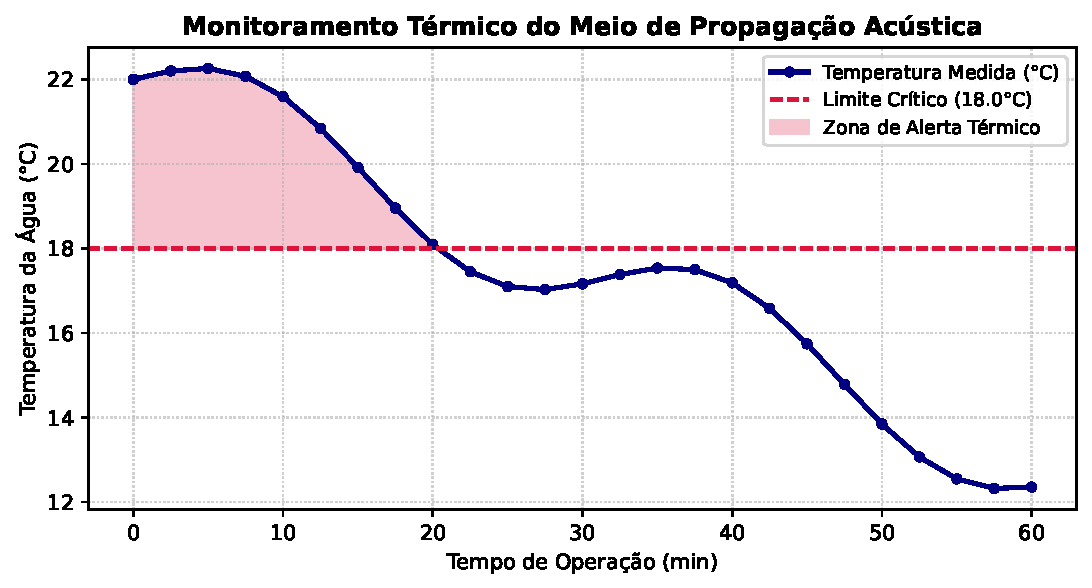
\includegraphics[width=0.88\linewidth]{body/Lista_12/figures/fig_Q9.pdf}
    \captionof{figure}{Saída gráfica gerada: curva temporal de temperatura com limiar crítico e zona de alerta sombreada.}
\end{center}
\fi


\vspace{0.5cm}

% Q10 - Aula 15: Matplotlib Dashboards com plt.subplots(1, 2)
\item \textbf{[Discursiva - 10,0 pontos]} No centro de controle de sonar de uma fragata, painéis analíticos sintéticos combinam distribuições estatísticas com contagens categóricas de contatos navais em múltiplos quadrantes táticos.

Implemente a função \code{gerar\_dashboard\_acustico(valores\_snr: List[float], setores: List[str], contagens: List[int], caminho\_img: str) -> bool} utilizando o \textbf{Matplotlib}:
\begin{itemize}[leftmargin=*]
    \item \textbf{1. Configuração da Grade de Subgráficos:}\newline
    Crie uma figura com uma linha e duas colunas de eixos com proporção panorâmica: \code{fig, (ax1, ax2) = plt.subplots(1, 2, figsize=(13, 5))}.
    \item \textbf{2. Painel Esquerdo (\code{ax1} - Histograma de SNR):}\newline
    \begin{itemize}
        \item Plote a distribuição de frequência dos valores de sinal-ruído (\code{valores\_snr}) usando \code{ax1.hist()} com $12$ intervalos (\emph{bins}), cor verde-azulado (\code{"teal"}), bordas pretas (\code{edgecolor="black"}) e transparência \code{0.75}.
        \item Calcule a média dos valores de SNR e adicione uma linha vertical tracejada vermelha com \code{ax1.axvline()} destacando o valor médio formatado com 1 casa decimal na legenda.
        \item Configure título (\code{"Distribuicao da Relacao Sinal-Ruido (SNR)"}), rótulos dos eixos com unidades (\code{"SNR (dB)"} e \code{"Frequencia de Deteccoes"}), grade pontilhada e legenda.
    \end{itemize}
    \item \textbf{3. Painel Direito (\code{ax2} - Gráfico de Barras com Rótulos Automáticos):}\newline
    \begin{itemize}
        \item Plote um gráfico de barras verticais com \code{ax2.bar(setores, contagens)}, cor azul-aço (\code{"steelblue"}), bordas pretas e largura \code{0.6}.
        \item Utilize o método moderno \code{ax2.bar\_label(barras, padding=3, fontweight="bold")} para exibir o valor numérico exato acima do topo de cada barra vertical.
        \item Configure título (\code{"Contatos Acusticos por Setor Tatico"}), rótulos dos eixos e grade apenas horizontal (\code{grid(axis="y")}).
    \end{itemize}
    \item \textbf{4. Ajuste e Salvamento Vetorial:}\newline
    Aplique \code{plt.tight\_layout()}, salve a figura em formato vetorial PDF no arquivo especificado por \code{caminho\_img} (ex: \code{"dashboard\_acustico.pdf"}) com \code{dpi=150} e \code{bbox\_inches="tight"}, encerre o objeto com \code{plt.close(fig)} e retorne \code{True}.
\end{itemize}

\begin{itemize}[leftmargin=*]
    \item \textbf{Protótipo:}\newline
    \code{from typing import List}\\\code{import matplotlib.pyplot as plt}\\\code{def gerar\_dashboard\_acustico(}\\\code{    valores\_snr: List[float],}\\\code{    setores: List[str],}\\\code{    contagens: List[int],}\\\code{    caminho\_img: str = "dashboard\_acustico.pdf"}\\\code{) -> bool:}
\end{itemize}

\ifmostrarGabarito
\begin{minted}{python}
import matplotlib.pyplot as plt
from typing import List

def gerar_dashboard_acustico(
    valores_snr: List[float],
    setores: List[str],
    contagens: List[int],
    caminho_img: str
) -> bool:
    """
    Renderiza painel com histograma de SNR e grafico de barras rotulado lado a lado.
    """
    # Cria grade de subgraficos 1 linha x 2 colunas com proporcao panoramica
    fig, (ax1, ax2) = plt.subplots(1, 2, figsize=(13, 5))
    
    # Subgrafico 1: Histograma de distribuicao da relacao sinal-ruido
    ax1.hist(valores_snr, bins=12, color="teal", edgecolor="black", alpha=0.75)
    media_snr = sum(valores_snr) / len(valores_snr) if valores_snr else 0.0
    ax1.axvline(media_snr, color="red", linestyle="--", linewidth=1.8, label=f"Media: {media_snr:.1f} dB")
    ax1.set_title("Distribuicao da Relacao Sinal-Ruido (SNR)", fontsize=11, fontweight="bold")
    ax1.set_xlabel("SNR (dB)", fontsize=10)
    ax1.set_ylabel("Frequencia de Deteccoes", fontsize=10)
    ax1.grid(True, linestyle=":", alpha=0.5)
    ax1.legend(loc="upper right")
    
    # Subgrafico 2: Grafico de barras verticais com contatos por setor
    barras = ax2.bar(setores, contagens, color="steelblue", edgecolor="black", width=0.6)
    # Adiciona rotulos numericos automaticos sobre o topo de cada barra
    ax2.bar_label(barras, padding=3, fontsize=9, fontweight="bold")
    ax2.set_title("Contatos Acusticos por Setor Tatico", fontsize=11, fontweight="bold")
    ax2.set_xlabel("Setor de Varredura", fontsize=10)
    ax2.set_ylabel("Total de Contatos", fontsize=10)
    ax2.grid(axis="y", linestyle=":", alpha=0.5)
    
    # Ajuste de margens, exportacao e fechamento
    plt.tight_layout()
    fig.savefig(caminho_img, dpi=150, bbox_inches="tight")
    plt.close(fig)
    return True
\end{minted}

\textbf{Explicação:}
A construção de *dashboards* no Matplotlib utiliza \texttt{plt.subplots(nrows, ncols)}, desempacotando os eixos em variáveis distintas (\texttt{ax1}, \texttt{ax2}). O método moderno \texttt{ax.bar\_label(barras)} automatiza a impressão de valores quantitativos acima das colunas, enquanto \texttt{plt.tight\_layout()} previne sobreposição de rótulos entre subgráficos adjacentes.

\vspace{0.2cm}
\begin{center}
    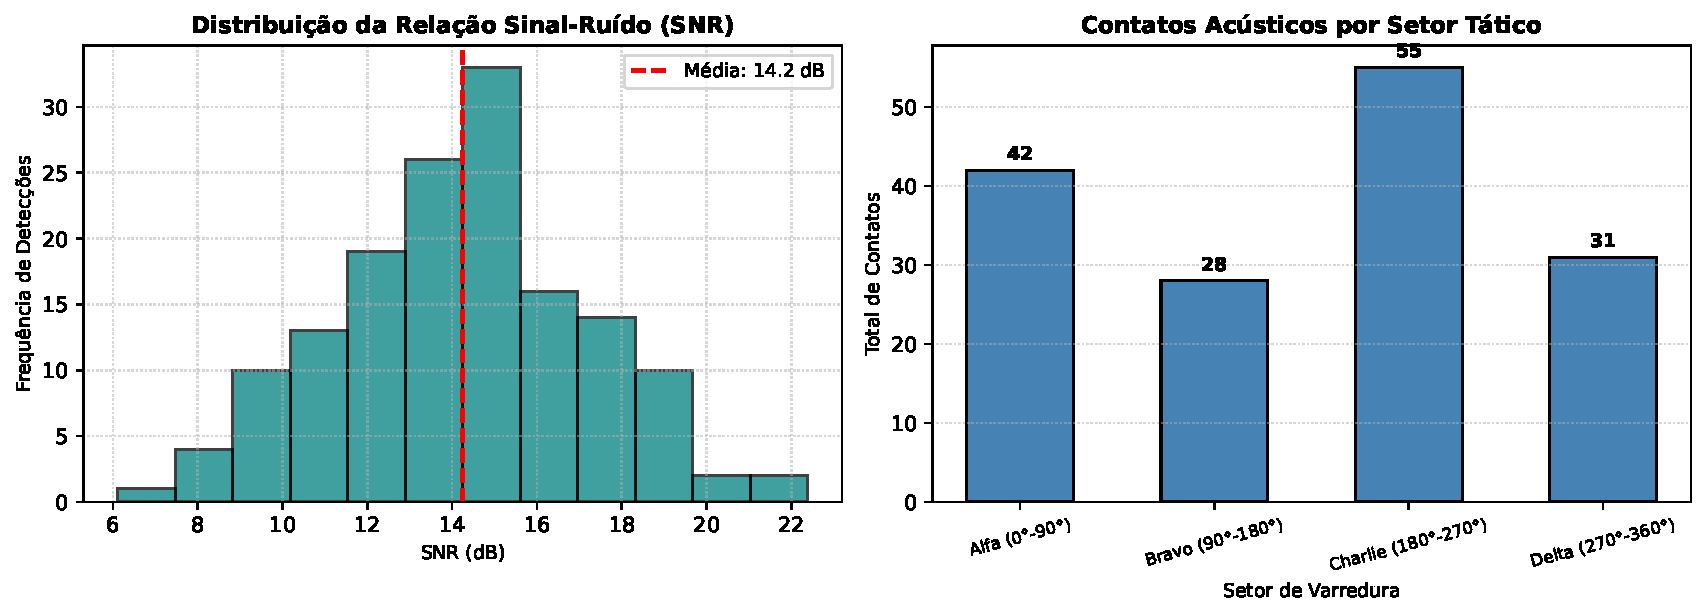
\includegraphics[width=0.98\linewidth]{body/Lista_12/figures/fig_Q10.pdf}
    \captionof{figure}{Dashboard acústico gerado: histograma de SNR com média vertical e gráfico de barras com contatos por setor.}
\end{center}
\fi


\end{enumerate}
